\documentclass{article} % For LaTeX2e
\usepackage{nips14submit_e,times}
\usepackage{amsmath}
\usepackage{amsthm}
\usepackage{amssymb}
\usepackage{mathtools}
\usepackage{hyperref}
\usepackage{url}
\usepackage{algorithm}
\usepackage[noend]{algpseudocode}
%\documentstyle[nips14submit_09,times,art10]{article} % For LaTeX 2.09

\usepackage{graphicx}
\usepackage{caption}
\usepackage{subcaption}

\def\eQb#1\eQe{\begin{eqnarray*}#1\end{eqnarray*}}
\def\eQnb#1\eQne{\begin{eqnarray}#1\end{eqnarray}}
\providecommand{\e}[1]{\ensuremath{\times 10^{#1}}}
\providecommand{\pb}[0]{\pagebreak}
\DeclarePairedDelimiter\ceil{\lceil}{\rceil}
\DeclarePairedDelimiter\floor{\lfloor}{\rfloor}

\newcommand{\E}{\mathrm{E}}
\newcommand{\Var}{\mathrm{Var}}
\newcommand{\Cov}{\mathrm{Cov}}

\def\Qb#1\Qe{\begin{question}#1\end{question}}
\def\Sb#1\Se{\begin{solution}#1\end{solution}}

\newenvironment{claim}[1]{\par\noindent\underline{Claim:}\space#1}{}
\newtheoremstyle{quest}{\topsep}{\topsep}{}{}{\bfseries}{}{ }{\thmname{#1}\thmnote{ #3}.}
\theoremstyle{quest}
\newtheorem*{definition}{Definition}
\newtheorem*{theorem}{Theorem}
\newtheorem*{lemma}{Lemma}
\newtheorem*{question}{Question}
\newtheorem*{preposition}{Preposition}
\newtheorem*{exercise}{Exercise}
\newtheorem*{challengeproblem}{Challenge Problem}
\newtheorem*{solution}{Solution}
\newtheorem*{remark}{Remark}
\usepackage{verbatimbox}
\usepackage{listings}
\title{Probabilistic Method: \\
Problem Set VI}


\author{
Youngduck Choi \\
CIMS \\
New York University\\
\texttt{yc1104@nyu.edu} \\
}


% The \author macro works with any number of authors. There are two commands
% used to separate the names and addresses of multiple authors: \And and \AND.
%
% Using \And between authors leaves it to \LaTeX{} to determine where to break
% the lines. Using \AND forces a linebreak at that point. So, if \LaTeX{}
% puts 3 of 4 authors names on the first line, and the last on the second
% line, try using \AND instead of \And before the third author name.

\newcommand{\fix}{\marginpar{FIX}}
\newcommand{\new}{\marginpar{NEW}}

\nipsfinalcopy % Uncomment for camera-ready version

\begin{document}


\maketitle

\begin{abstract}
This work contains solutions to the problem set VI
of Probabilistic Method 2016 at Courant Institute of Mathematical Sciences.
\end{abstract}

\bigskip

\begin{question}[2]
\hfill
\begin{figure}[h!]
  \centering
    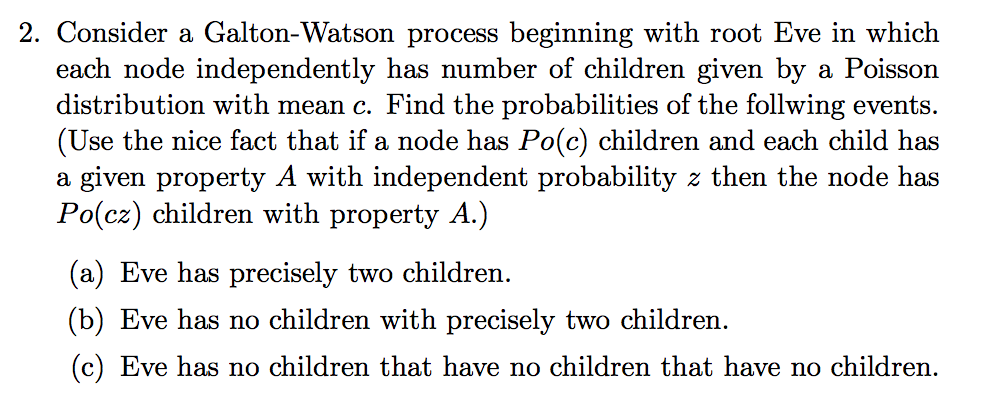
\includegraphics[width=0.7\textwidth]{pm-6-1.png}
\end{figure}
\end{question}
\begin{solution} \hfill \\
\textbf{(a)} As the number of children for each node is given by the Poisson distribution,
we have that the probability of Eve having precisely two children given by
\eQb
P(\{ \text{ Eve has precisely two children } \} ) &=& e^{-c}\dfrac{c^2}{2!}.
\eQe

\bigskip

\textbf{(b)} From the above computation, we see
that the event of each child having precisely two children has independent 
probability of 
$e^{-c}\dfrac{c^2}{2!}$. Therefore, using the useful fact, we have 
\eQb
P(\{ \text{ Eve has no children with precisely two children }
\}) &=& e^{-cz} \\
&=& e^{-c e^{-c}\frac{c^2}{2!}}.
\eQe 

\bigskip

\textbf{(c)}
We proceed by the same method. We again see that the event of each child 
having no children has independent probability of $e^{-c}$. Therefore,
by the useful fact, we have
\eQb
P( \{ \text{ A node has no children that hve no children } \} ) &=& e^{-c e^{-c}}.  
\eQe
Using the same argument once more, we obtain
\eQb
P( \{ \text{ Eve has no children that have no children that have no children} \} ) &=& e^{-ce^{-c e^{-c}}}.  
\eQe
\hfill $\qed$
\end{solution}

\newpage

\begin{question}[2]
\hfill
\begin{figure}[h!]
  \centering
    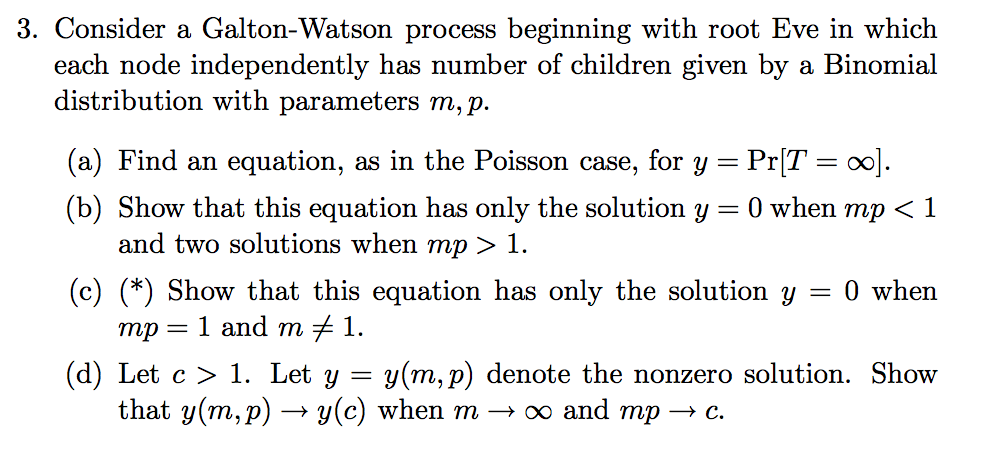
\includegraphics[width=0.8\textwidth]{pm-6-2.png}
\end{figure}
\end{question}
\begin{solution}
\textbf{(a)} Let $y = Pr[T = \infty]$, and $z = Pr[T < \infty] = 1 - y$. By partitioning the space
with the number of children that Eve has, and using the fact that the sub-tree must be finite, we obtain
\eQb
z &=& \sum_{i=0}^{m} {m \choose i} p^i (1-p)^{m-i} z^i \\
&=& (pz + 1 - p)^{m},
\eQe 
thus
\eQb
1 - y &=& [1-py]^m.
\eQe

\bigskip

\textbf{(b)}
Now, we view the problem of finding solutions to the above equation as finding intersections
of the graphs $f(y) = 1 - y$ and $g(y) =(1-py)^{m}$ with $p,m$ as parameters within the domain
$y \in [0,1]$. 
Observe that for any $p,m$, we 
trivially have $y = 0$ as a solution. Furthermore, observe that $g'(y) = -mp(1-py)^{m-1}$, 
and $g''(y) = m(m-1)p^2(1-py)^{m-2}$. As $p$ and
$y$ are both probabilities, $1-py$ is always non-negative, and we have that $g$ is convex. Hence,
we can deduce that there are at most one more solution, other than $y = 0$. 
Now, as $g'(0) = -mp$ and $f'(0) = -1$, if $mp < 1$, it follows that $f'(0) < g'(0)$. This implies 
that there will be no other intersection. Similarly, if $mp > 1$, we have $f'(0) > g'(0)$, and
as $f(1) < g(1)$. By intermediate value theorem, we must have a crossing between $f$ and $g$.
Therefore, if $mp > 1$, there are two solutions.  
 
\bigskip

\textbf{(c)} Now, $mp = 1$ with $m \neq 1$, which implies that $p \neq 1$. From the above
analysis, we have that $g'(0) = -mp$ and this cases shows that $f$ is a tangent line
of $g$ precisely at $0$. Again, by convexity, the graph cannot intersect at any other point. 

\bigskip

\textbf{(d)}
Let $y(c)$ be the unique positive $y$ with $e^{-cy} = 1-y$, and let $f_m(y) = (1-py)^m$. 
With $p = \frac{c}{m}$, we have
\eQb
1 -y &=& \lim_{m \to \infty} (1- \frac{cy}{m})^{m} = e^{-cy}, 
\eQe
by elementary analysis. As $y(c)$ is the solution to $1-y = e^{-cy}$, it follows that
for $m$ large enough, we have $(1 - \frac{cy}{m})^{m} - y(c)$ is small. 
Hence, we have shown that  the solution of $1-y = (1-py)^{m}$ goes to $y(c)$ in the limit.
\hfill $\qed$


\end{solution}

\newpage

\end{document}

